\clearemptydoublepage
\chapter{Contexte}

\section{Cloud computing}

\subsection{Caractéristiques}

\begin{figure}[htbp]
    \centering
	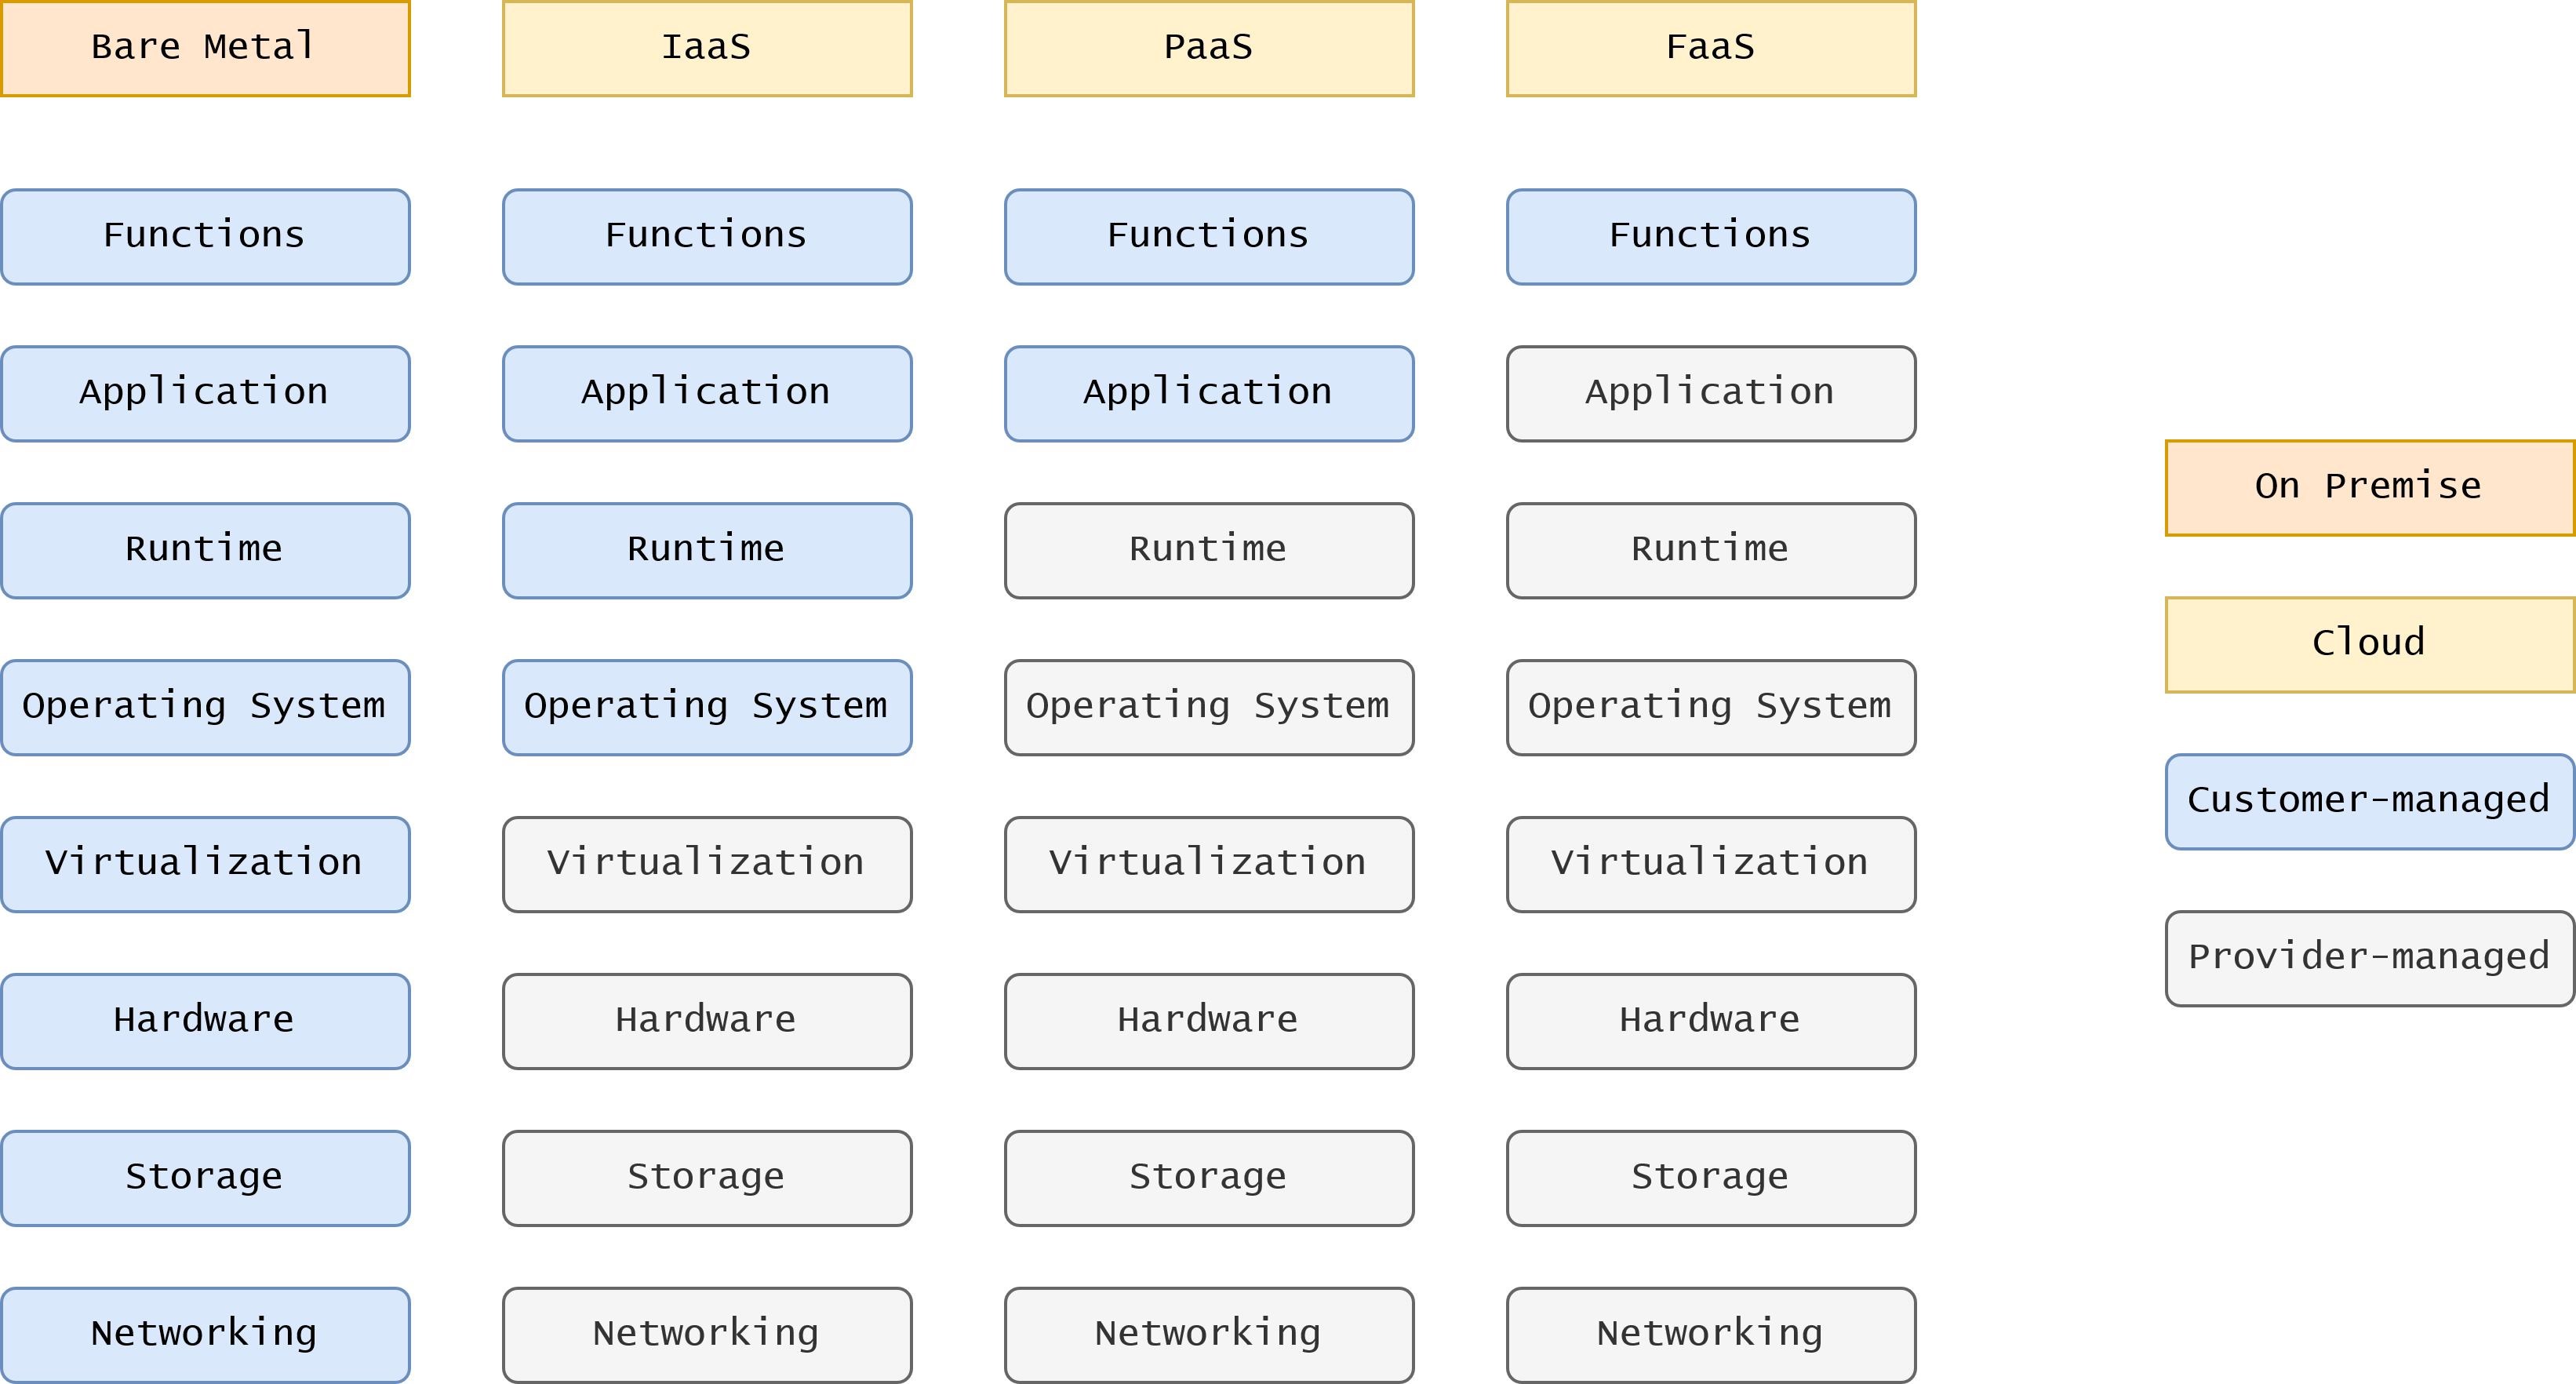
\includegraphics[width=\textwidth]{3_Chapitre1/figures/service-models.png}
	\caption[Comparaison entre différents modèles de service pour le cloud en termes de responsabilités pour le client et le fournisseur de service.]{Comparaison entre différents modèles de service pour le cloud en termes de responsabilités pour le client et le fournisseur de service (inspiré de la documentation Red Hat \protect \footnotemark).}
	\label{fig:service-model}
\end{figure}

\footnotetext{\url{https://www.redhat.com/en/topics/cloud-computing/iaas-vs-paas-vs-saas}}

Le NIST donne une définition formelle du cloud~\cite{mellNISTDefinitionCloud} en listant les caractéristiques essentielles d'une telle plateforme :

\begin{itemize}
    \item \textbf{Service à la demande} -- Les clients réservent des ressources matérielles de manière autonome, par exemple au travers d'une interface web, sans interagir avec un opérateur. En retour, ils n'ont généralement pas de contrôle fin sur la localité précise des ressources réservées ;
    \item \textbf{Accessible par le réseau} -- Ces ressources sont immédiatement mises à disposition des clients et accessibles par Internet ;
    \item \textbf{Partage des ressources} -- La puissance de calcul, les capacités de stockage et la bande passante sont partagées entre les clients du fournisseur de services. Des techniques de virtualisation sont mises en œuvre pour isoler les tâches déployées ;
    \item \textbf{Élasticité rapide} -- Les clients peuvent à tout moment décider d'augmenter ou de diminuer la quantité et les caractéristiques des ressources qu'ils réservent, de manière à garantir les performances de leurs applications ou maîtriser leurs coûts ;
    \item \textbf{Service mesuré} -- Les infrastructures cloud sont instrumentées de manière à fournir aux clients une information précise sur leur consommation de ressources, et les coûts monétaires associés.
\end{itemize}

\subsection{Modèles de service}

Ces caractéristiques sont déclinées dans trois modèles de service :

\begin{itemize}
    \item \textbf{Software as a Service} (SaaS) -- Cible l'utilisateur final en offrant l'accès à une application entièrement administrée par le fournisseur de services ;
    \item \textbf{Platform as a Service} (PaaS) -- Cible les clients qui souhaitent déployer leurs applications sans avoir la responsabilité d'administration des serveurs ;
    \item \textbf{Infrastructure as a Service} (IaaS) -- Cible les clients qui souhaitent un contrôle à grain fin sur leurs infrastructures. Les clients d'une offre IaaS sont responsables de l'administration de leurs serveurs, souvent virtuels. 
\end{itemize}

\subsection{Modèles de déploiement}

Enfin, ...

\begin{itemize}
    \item \textbf{Cloud privé} -- L'infrastructure est dédiée à une organisation qui regroupe plusieurs utilisateurs finaux. Ce modèle de déploiement est privilégié pour la sécurité et la confidentialité des données ;
    \item \textbf{Cloud public} -- L'infrastructure est partagée entre de nombreux clients hétérogènes, professionnels comme particuliers ;
    \item \textbf{Cloud communautaire} -- L'infrastructure est partagée entre différents acteurs ayant souvent des problématiques métier similaires (secteurs bancaire ou hospitalier par exemple) ;
    \item \textbf{Cloud hybride} -- Solution de répartition des tâches entre cloud privé et cloud public, en fonction de leur niveau de criticité.
\end{itemize}

\section{Ordonnancement dans le cloud}

\subsection{Virtualisation dans un cadre multi-tenant}

\subsection{Dimensionnement et passage à l'échelle}

\subsection{Qualité de service et métriques de performances}

Problème : overbooking, overcommitting... conso d'énergie...

\section{Applications dans le cloud}

\subsection{Du monolithe aux micro-services}

\subsection{Développement cloud-native}

\subsection{Vers un nouveau modèle de service}

\section{Conclusion}
